\documentclass{standalone}
\usepackage{tikz}
\usetikzlibrary{patterns, positioning}


\begin{document}
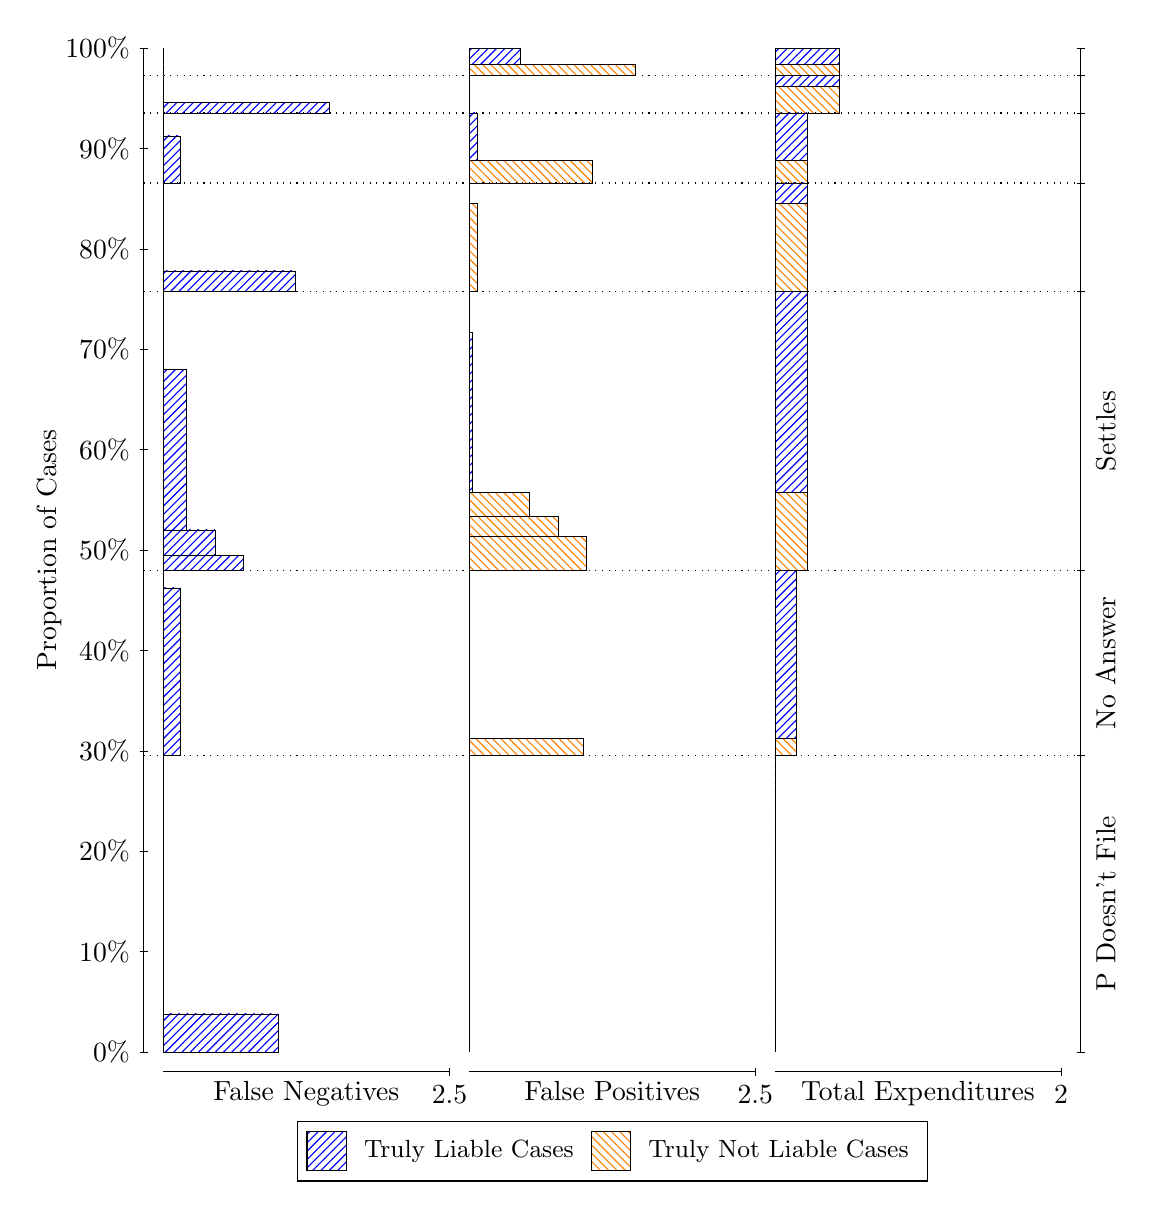
\begin{tikzpicture}
\draw[black, very thin] (1.5,1.75) -- (1.5,14.5);
\node[rotate=90, text=black, anchor=center] at (0.3, 8.125) {Proportion of Cases};
\draw[black, very thin] (1.45,1.75) -- (1.55,1.75);
\node[text=black, anchor=east] at (1.45, 1.75) {0\%};
\draw[black, very thin] (1.45,3.025) -- (1.55,3.025);
\node[text=black, anchor=east] at (1.45, 3.025) {10\%};
\draw[black, very thin] (1.45,4.3) -- (1.55,4.3);
\node[text=black, anchor=east] at (1.45, 4.3) {20\%};
\draw[black, very thin] (1.45,5.575) -- (1.55,5.575);
\node[text=black, anchor=east] at (1.45, 5.575) {30\%};
\draw[black, very thin] (1.45,6.85) -- (1.55,6.85);
\node[text=black, anchor=east] at (1.45, 6.85) {40\%};
\draw[black, very thin] (1.45,8.125) -- (1.55,8.125);
\node[text=black, anchor=east] at (1.45, 8.125) {50\%};
\draw[black, very thin] (1.45,9.4) -- (1.55,9.4);
\node[text=black, anchor=east] at (1.45, 9.4) {60\%};
\draw[black, very thin] (1.45,10.675) -- (1.55,10.675);
\node[text=black, anchor=east] at (1.45, 10.675) {70\%};
\draw[black, very thin] (1.45,11.95) -- (1.55,11.95);
\node[text=black, anchor=east] at (1.45, 11.95) {80\%};
\draw[black, very thin] (1.45,13.225) -- (1.55,13.225);
\node[text=black, anchor=east] at (1.45, 13.225) {90\%};
\draw[black, very thin] (1.45,14.5) -- (1.55,14.5);
\node[text=black, anchor=east] at (1.45, 14.5) {100\%};

\draw[black, very thin] (13.4,1.75) -- (13.4,14.5);
\draw[black, very thin] (13.35,1.75) -- (13.45,1.75);
\node[anchor=west] at (13.35, 1.75) {};
\draw[black, very thin] (13.35,5.5119) -- (13.45,5.5119);
\node[anchor=west] at (13.35, 5.5119) {};
\draw[black, very thin] (13.35,7.8664) -- (13.45,7.8664);
\node[anchor=west] at (13.35, 7.8664) {};
\draw[black, very thin] (13.35,11.406) -- (13.45,11.406);
\node[anchor=west] at (13.35, 11.406) {};
\draw[black, very thin] (13.35,12.786) -- (13.45,12.786);
\node[anchor=west] at (13.35, 12.786) {};
\draw[black, very thin] (13.35,13.675) -- (13.45,13.675);
\node[anchor=west] at (13.35, 13.675) {};
\draw[black, very thin] (13.35,14.154) -- (13.45,14.154);
\node[anchor=west] at (13.35, 14.154) {};
\draw[black, very thin] (13.35,14.5) -- (13.45,14.5);
\node[anchor=west] at (13.35, 14.5) {};

\draw[black, very thin, pattern color=blue, pattern=north east lines] (1.75,1.75) rectangle (3.2033,2.2345);
\draw[black, very thin, pattern color=orange, pattern=north west lines] (1.75,2.2345) rectangle (1.75,5.5119);
\draw[black, very thin, pattern color=blue, pattern=north east lines] (1.75,5.5119) rectangle (1.968,7.6446);
\draw[black, very thin, pattern color=orange, pattern=north west lines] (1.75,7.6446) rectangle (1.75,7.8664);
\draw[black, very thin, pattern color=blue, pattern=north east lines] (1.75,7.8664) rectangle (2.7673,8.0592);
\draw[black, very thin, pattern color=blue, pattern=north east lines] (1.75,8.0592) rectangle (2.404,8.3806);
\draw[black, very thin, pattern color=blue, pattern=north east lines] (1.75,8.3806) rectangle (2.0407,10.416);
\draw[black, very thin, pattern color=orange, pattern=north west lines] (1.75,10.416) rectangle (1.75,11.406);
\draw[black, very thin, pattern color=blue, pattern=north east lines] (1.75,11.406) rectangle (3.4213,11.669);
\draw[black, very thin, pattern color=orange, pattern=north west lines] (1.75,11.669) rectangle (1.75,12.786);
\draw[black, very thin, pattern color=blue, pattern=north east lines] (1.75,12.786) rectangle (1.968,13.385);
\draw[black, very thin, pattern color=orange, pattern=north west lines] (1.75,13.385) rectangle (1.75,13.675);
\draw[black, very thin, pattern color=blue, pattern=north east lines] (1.75,13.675) rectangle (3.8573,13.813);
\draw[black, very thin, pattern color=orange, pattern=north west lines] (1.75,13.813) rectangle (1.75,14.154);
\draw[black, very thin, pattern color=orange, pattern=north west lines] (1.75,14.154) rectangle (1.75,14.293);
\draw[black, very thin, pattern color=blue, pattern=north east lines] (1.75,14.293) rectangle (1.75,14.5);
\draw[black, very thin, pattern color=orange, pattern=north west lines] (5.6333,1.75) rectangle (5.6333,5.0274);
\draw[black, very thin, pattern color=blue, pattern=north east lines] (5.6333,5.0274) rectangle (5.6333,5.5119);
\draw[black, very thin, pattern color=orange, pattern=north west lines] (5.6333,5.5119) rectangle (7.0867,5.7336);
\draw[black, very thin, pattern color=blue, pattern=north east lines] (5.6333,5.7336) rectangle (5.6333,7.8664);
\draw[black, very thin, pattern color=orange, pattern=north west lines] (5.6333,7.8664) rectangle (7.123,8.2937);
\draw[black, very thin, pattern color=orange, pattern=north west lines] (5.6333,8.2937) rectangle (6.7597,8.5471);
\draw[black, very thin, pattern color=orange, pattern=north west lines] (5.6333,8.5471) rectangle (6.3963,8.8562);
\draw[black, very thin, pattern color=blue, pattern=north east lines] (5.6333,8.8562) rectangle (5.6697,10.892);
\draw[black, very thin, pattern color=blue, pattern=north east lines] (5.6333,10.892) rectangle (5.6333,11.406);
\draw[black, very thin, pattern color=orange, pattern=north west lines] (5.6333,11.406) rectangle (5.7423,12.523);
\draw[black, very thin, pattern color=blue, pattern=north east lines] (5.6333,12.523) rectangle (5.6333,12.786);
\draw[black, very thin, pattern color=orange, pattern=north west lines] (5.6333,12.786) rectangle (7.1957,13.075);
\draw[black, very thin, pattern color=blue, pattern=north east lines] (5.6333,13.075) rectangle (5.7423,13.675);
\draw[black, very thin, pattern color=orange, pattern=north west lines] (5.6333,13.675) rectangle (5.6333,14.015);
\draw[black, very thin, pattern color=blue, pattern=north east lines] (5.6333,14.015) rectangle (5.6333,14.154);
\draw[black, very thin, pattern color=orange, pattern=north west lines] (5.6333,14.154) rectangle (7.7407,14.293);
\draw[black, very thin, pattern color=blue, pattern=north east lines] (5.6333,14.293) rectangle (6.2873,14.5);
\draw[black, very thin, pattern color=orange, pattern=north west lines] (9.5167,1.75) rectangle (9.5167,5.0274);
\draw[black, very thin, pattern color=blue, pattern=north east lines] (9.5167,5.0274) rectangle (9.5167,5.5119);
\draw[black, very thin, pattern color=orange, pattern=north west lines] (9.5167,5.5119) rectangle (9.7892,5.7336);
\draw[black, very thin, pattern color=blue, pattern=north east lines] (9.5167,5.7336) rectangle (9.7892,7.8664);
\draw[black, very thin, pattern color=orange, pattern=north west lines] (9.5167,7.8664) rectangle (9.9254,8.8562);
\draw[black, very thin, pattern color=blue, pattern=north east lines] (9.5167,8.8562) rectangle (9.9254,11.406);
\draw[black, very thin, pattern color=orange, pattern=north west lines] (9.5167,11.406) rectangle (9.9254,12.523);
\draw[black, very thin, pattern color=blue, pattern=north east lines] (9.5167,12.523) rectangle (9.9254,12.786);
\draw[black, very thin, pattern color=orange, pattern=north west lines] (9.5167,12.786) rectangle (9.9254,13.075);
\draw[black, very thin, pattern color=blue, pattern=north east lines] (9.5167,13.075) rectangle (9.9254,13.675);
\draw[black, very thin, pattern color=orange, pattern=north west lines] (9.5167,13.675) rectangle (10.334,14.015);
\draw[black, very thin, pattern color=blue, pattern=north east lines] (9.5167,14.015) rectangle (10.334,14.154);
\draw[black, very thin, pattern color=orange, pattern=north west lines] (9.5167,14.154) rectangle (10.334,14.293);
\draw[black, very thin, pattern color=blue, pattern=north east lines] (9.5167,14.293) rectangle (10.334,14.5);
\draw[black, dotted] (1.5,5.5119) -- (13.4,5.5119);
\draw[black, dotted] (1.5,7.8664) -- (13.4,7.8664);
\draw[black, dotted] (1.5,11.406) -- (13.4,11.406);
\draw[black, dotted] (1.5,12.786) -- (13.4,12.786);
\draw[black, dotted] (1.5,13.675) -- (13.4,13.675);
\draw[black, dotted] (1.5,14.154) -- (13.4,14.154);
\draw[black, very thin] (1.75,1.5) -- (5.3833,1.5);
\node[text=black, anchor=north] at (3.5667, 1.5) {False Negatives};
\draw[black, very thin] (5.3833,1.45) -- (5.3833,1.55);
\node[text=black, anchor=north] at (5.3833, 1.45) {2.5};

\draw[black, very thin] (5.6333,1.5) -- (9.2667,1.5);
\node[text=black, anchor=north] at (7.45, 1.5) {False Positives};
\draw[black, very thin] (9.2667,1.45) -- (9.2667,1.55);
\node[text=black, anchor=north] at (9.2667, 1.45) {2.5};

\draw[black, very thin] (9.5167,1.5) -- (13.15,1.5);
\node[text=black, anchor=north] at (11.333, 1.5) {Total Expenditures};
\draw[black, very thin] (13.15,1.45) -- (13.15,1.55);
\node[text=black, anchor=north] at (13.15, 1.45) {2};

\node[text=black, centered, rotate=90] at (13.72, 3.6309) {P Doesn't File};
\node[text=black, centered, rotate=90] at (13.72, 6.6891) {No Answer};
\node[text=black, centered, rotate=90] at (13.72, 9.6363) {Settles};





\draw (7.449999999999999,1.5) node[draw=none] (baseCoordinate) {};
\begin{scope}[align=center]
        \matrix[scale=0.5, draw=black, below=0.5cm of baseCoordinate, nodes={draw}, column sep=0.1cm]{
            \node[rectangle, draw, minimum width=0.5cm, minimum height=0.5cm, pattern color=blue, pattern=north east lines] {}; &
            \node[draw=none, font=\small, text=black] (B) {Truly Liable Cases}; &
            \node[rectangle, draw, minimum width=0.5cm, minimum height=0.5cm, pattern color=orange, pattern=north west lines] {}; &
            \node[draw=none, font=\small, text=black] (B) {Truly Not Liable Cases}; \\
            };
\end{scope}

\end{tikzpicture}
\end{document}